% Reconstructed cube options: preserve the printed vertex and line incidence,
% but do not infer metric proportions from the perspective drawing.
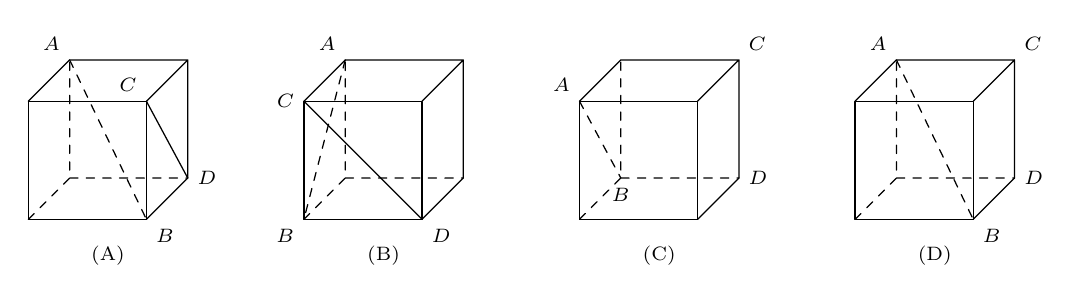
\begin{tikzpicture}[x=.75cm,y=.75cm,line cap=round,line join=round]
\tikzset{cube edge/.style={line width=.45pt}, hidden edge/.style={cube edge,dashed}}

% (A): A=back TL, C=front TR, B=front BR, D=back BR.
\begin{scope}
  \coordinate (a) at (0,0); \coordinate (b) at (2,0);
  \coordinate (c) at (2,2); \coordinate (d) at (0,2);
  \coordinate (e) at (.7,.7); \coordinate (f) at (2.7,.7);
  \coordinate (g) at (2.7,2.7); \coordinate (h) at (.7,2.7);
  \draw[cube edge] (a)--(b)--(c)--(d)--cycle;
  \draw[cube edge] (d)--(h)--(g)--(c) (g)--(f)--(b);
  \draw[hidden edge] (a)--(e)--(h) (e)--(f);
  \draw[hidden edge] (h)--(b);
  \draw[cube edge] (c)--(f);
  \node[font=\scriptsize,above left] at (h) {$A$};
  \node[font=\scriptsize,above left] at (c) {$C$};
  \node[font=\scriptsize,below right] at (b) {$B$};
  \node[font=\scriptsize,right] at (f) {$D$};
  \node[font=\scriptsize] at (1.35,-.62) {(A)};
\end{scope}

% (B): A=back TL, C=front TL, B=front BL, D=front BR.
\begin{scope}[xshift=3.5cm]
  \coordinate (a) at (0,0); \coordinate (b) at (2,0);
  \coordinate (c) at (2,2); \coordinate (d) at (0,2);
  \coordinate (e) at (.7,.7); \coordinate (f) at (2.7,.7);
  \coordinate (g) at (2.7,2.7); \coordinate (h) at (.7,2.7);
  \draw[cube edge] (a)--(b)--(c)--(d)--cycle;
  \draw[cube edge] (d)--(h)--(g)--(c) (g)--(f)--(b);
  \draw[hidden edge] (a)--(e)--(h) (e)--(f);
  \draw[hidden edge] (h)--(a);
  \draw[cube edge] (d)--(b);
  \node[font=\scriptsize,above left] at (h) {$A$};
  \node[font=\scriptsize,left] at (d) {$C$};
  \node[font=\scriptsize,below left] at (a) {$B$};
  \node[font=\scriptsize,below right] at (b) {$D$};
  \node[font=\scriptsize] at (1.35,-.62) {(B)};
\end{scope}

% (C): A=front TL, C=back TR, B=back BL, D=back BR.
\begin{scope}[xshift=7cm]
  \coordinate (a) at (0,0); \coordinate (b) at (2,0);
  \coordinate (c) at (2,2); \coordinate (d) at (0,2);
  \coordinate (e) at (.7,.7); \coordinate (f) at (2.7,.7);
  \coordinate (g) at (2.7,2.7); \coordinate (h) at (.7,2.7);
  \draw[cube edge] (a)--(b)--(c)--(d)--cycle;
  \draw[cube edge] (d)--(h)--(g)--(c) (g)--(f)--(b);
  \draw[hidden edge] (a)--(e)--(h) (e)--(f);
  \draw[hidden edge] (d)--(e);
  \node[font=\scriptsize,above left] at (d) {$A$};
  \node[font=\scriptsize,above right] at (g) {$C$};
  \node[font=\scriptsize,below] at (e) {$B$};
  \node[font=\scriptsize,right] at (f) {$D$};
  \node[font=\scriptsize] at (1.35,-.62) {(C)};
\end{scope}

% (D): A=back TL, C=back TR, B=front BR, D=back BR.
\begin{scope}[xshift=10.5cm]
  \coordinate (a) at (0,0); \coordinate (b) at (2,0);
  \coordinate (c) at (2,2); \coordinate (d) at (0,2);
  \coordinate (e) at (.7,.7); \coordinate (f) at (2.7,.7);
  \coordinate (g) at (2.7,2.7); \coordinate (h) at (.7,2.7);
  \draw[cube edge] (a)--(b)--(c)--(d)--cycle;
  \draw[cube edge] (d)--(h)--(g)--(c) (g)--(f)--(b);
  \draw[hidden edge] (a)--(e)--(h) (e)--(f);
  \draw[hidden edge] (h)--(b);
  \draw[cube edge] (g)--(f);
  \node[font=\scriptsize,above left] at (h) {$A$};
  \node[font=\scriptsize,above right] at (g) {$C$};
  \node[font=\scriptsize,below right] at (b) {$B$};
  \node[font=\scriptsize,right] at (f) {$D$};
  \node[font=\scriptsize] at (1.35,-.62) {(D)};
\end{scope}
\end{tikzpicture}
